\subsection{Space Confinement}

For this module, we successfully configured the drone to receive and decode the navigation data packages that were being sent from the drone to the laptop. The three datasets which were useful to this module are shown in Figure \ref{fig:4c-sample-nav}.

\begin{figure}[H]
      \centering
      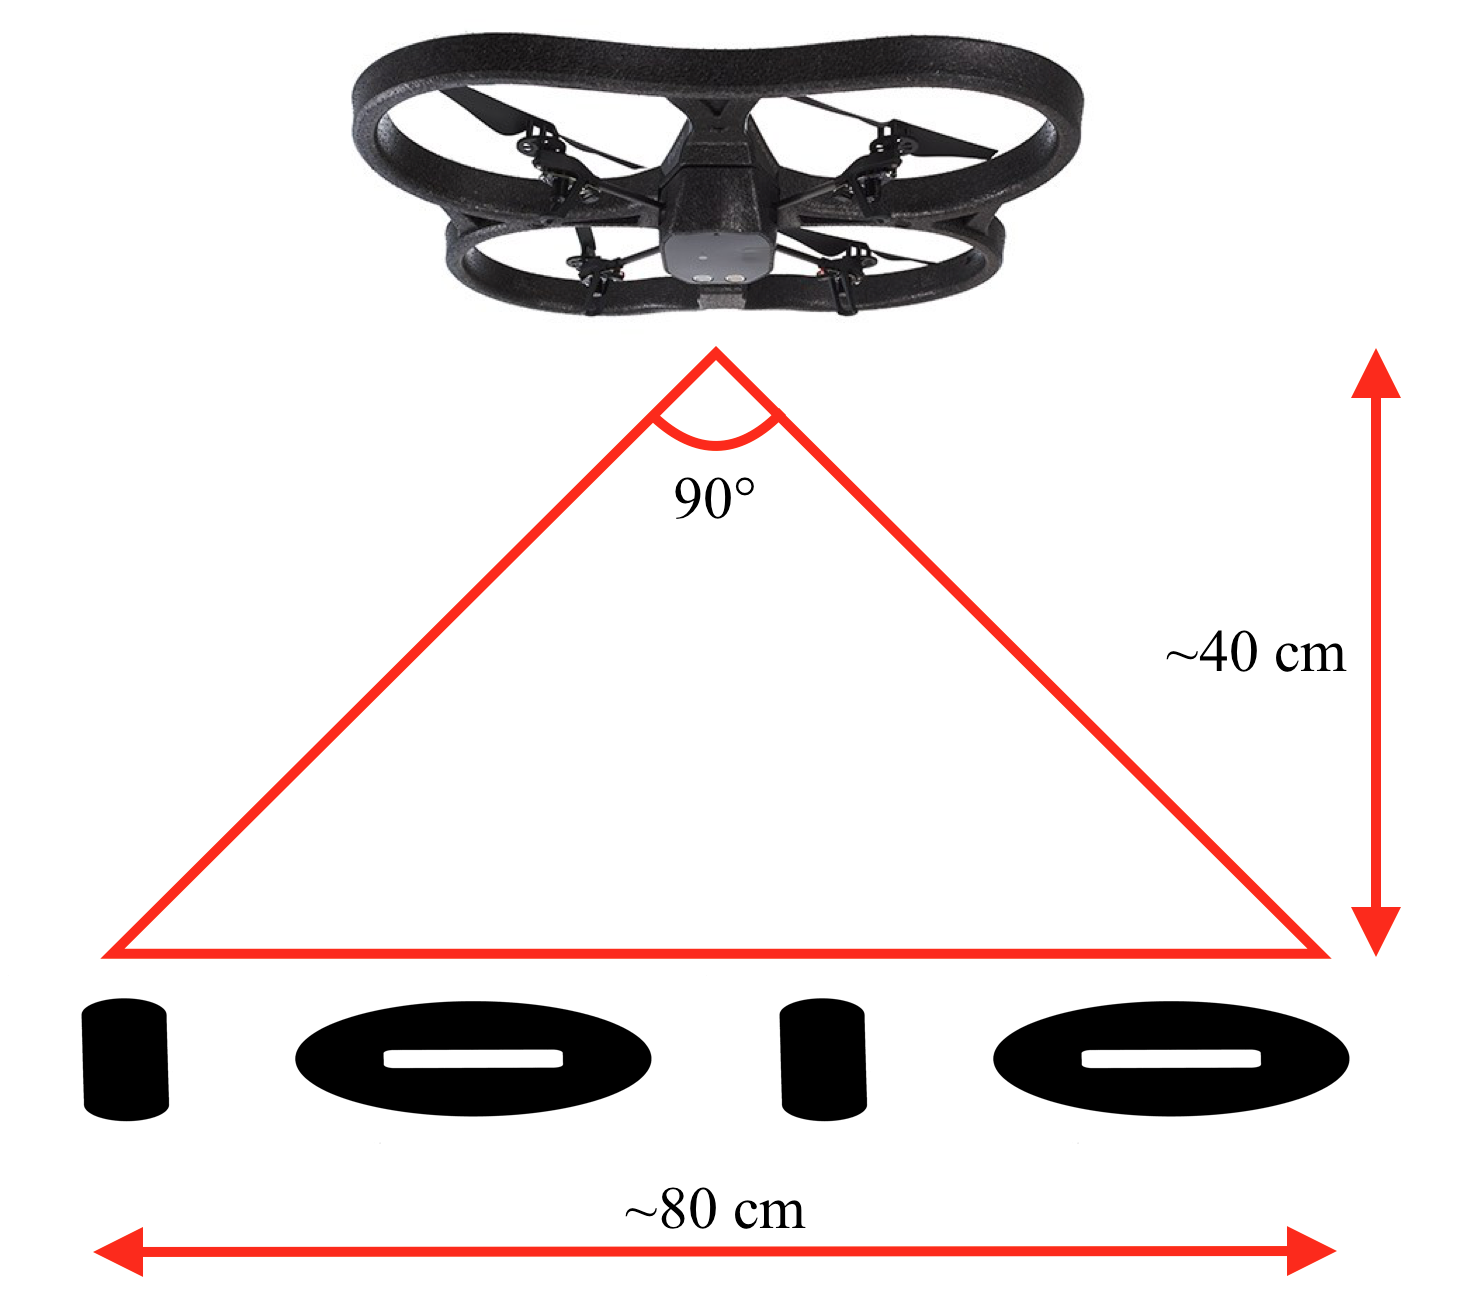
\includegraphics[width=0.8\linewidth]{3d-drone-fov.png}
      \caption{Sample navigation data from the drone when rotating clockwise near a roundel}
      \label{fig:4c-sample-nav}
\end{figure}

The following figure includes a few screenshots from a video where the drone approaches a row of roundels, and then backs away again.

\onecolumn
\begin{figure}
        \begin{subfigure}[b]{0.25\textwidth}
                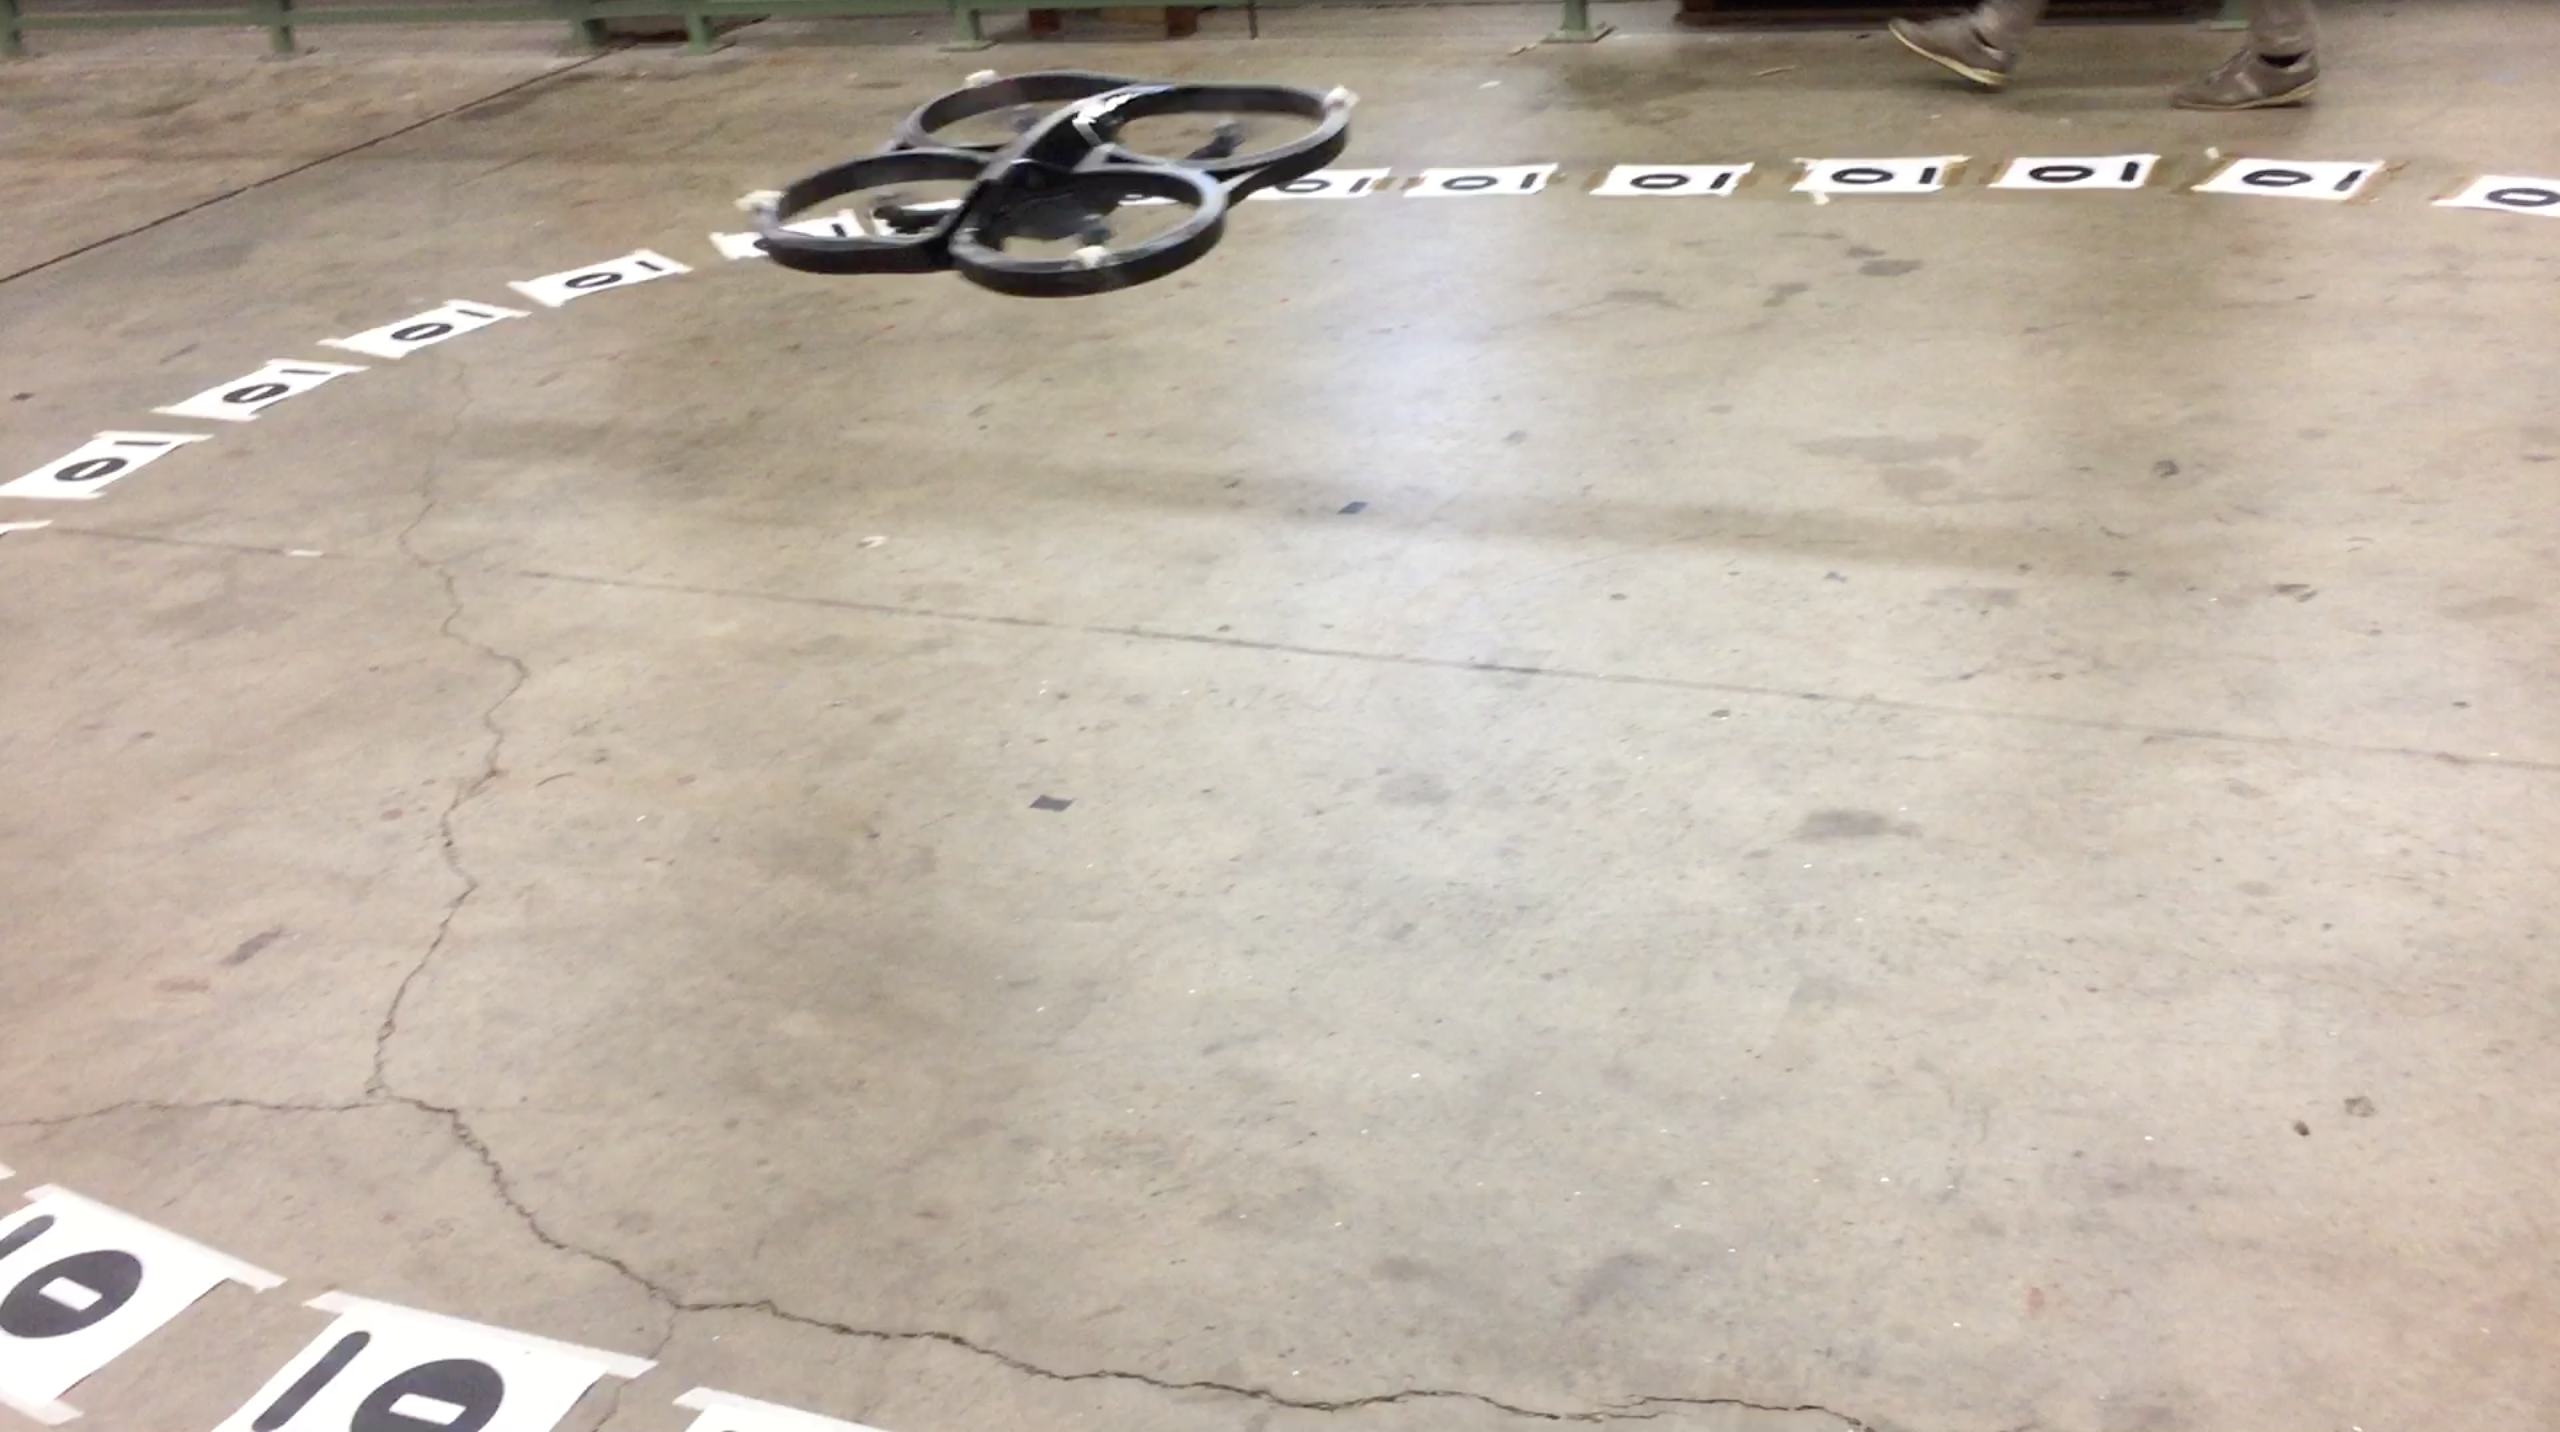
\includegraphics[width=\linewidth]{4c-flying-towards.png}
                \caption{Drone is flying towards the roundel boundary}
        \end{subfigure}%
        \hspace{\fill}
        \begin{subfigure}[b]{0.25\textwidth}
                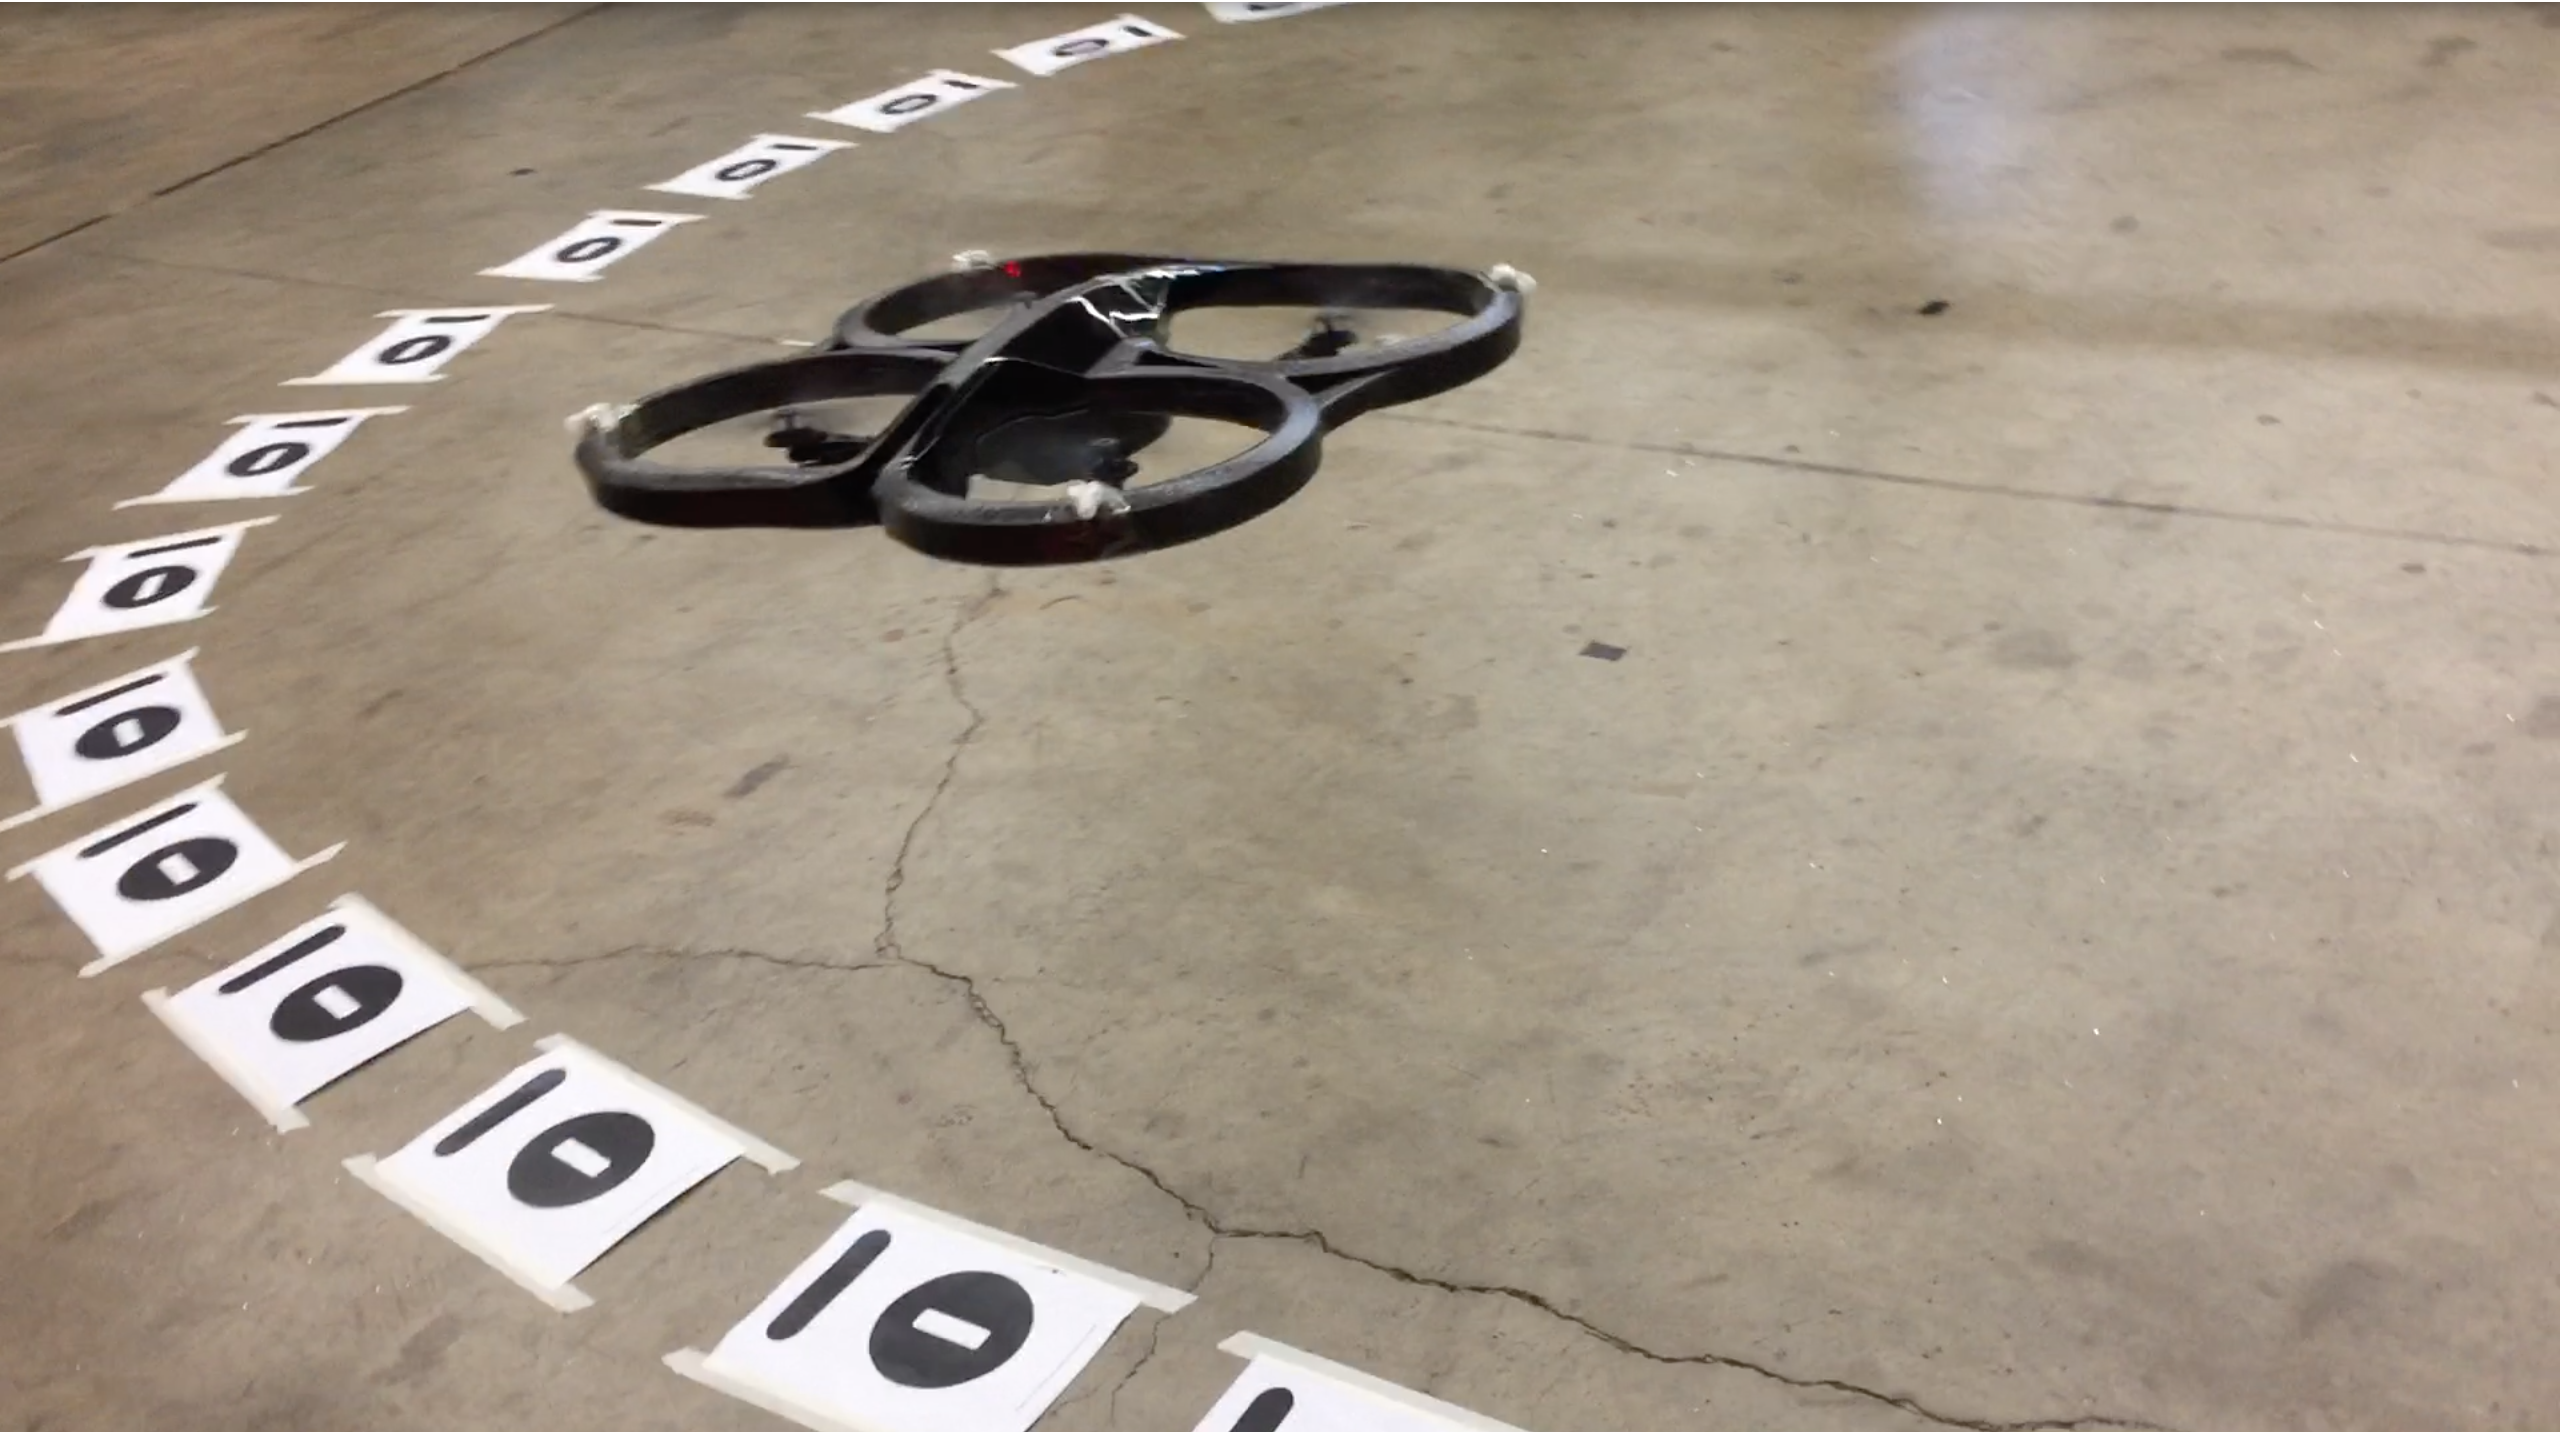
\includegraphics[width=\linewidth]{4c-found-boundary.png}
                \caption{Drone has detected a roundel at the boundary}
        \end{subfigure}%
        \hspace{\fill}
        \begin{subfigure}[b]{0.25\textwidth}
                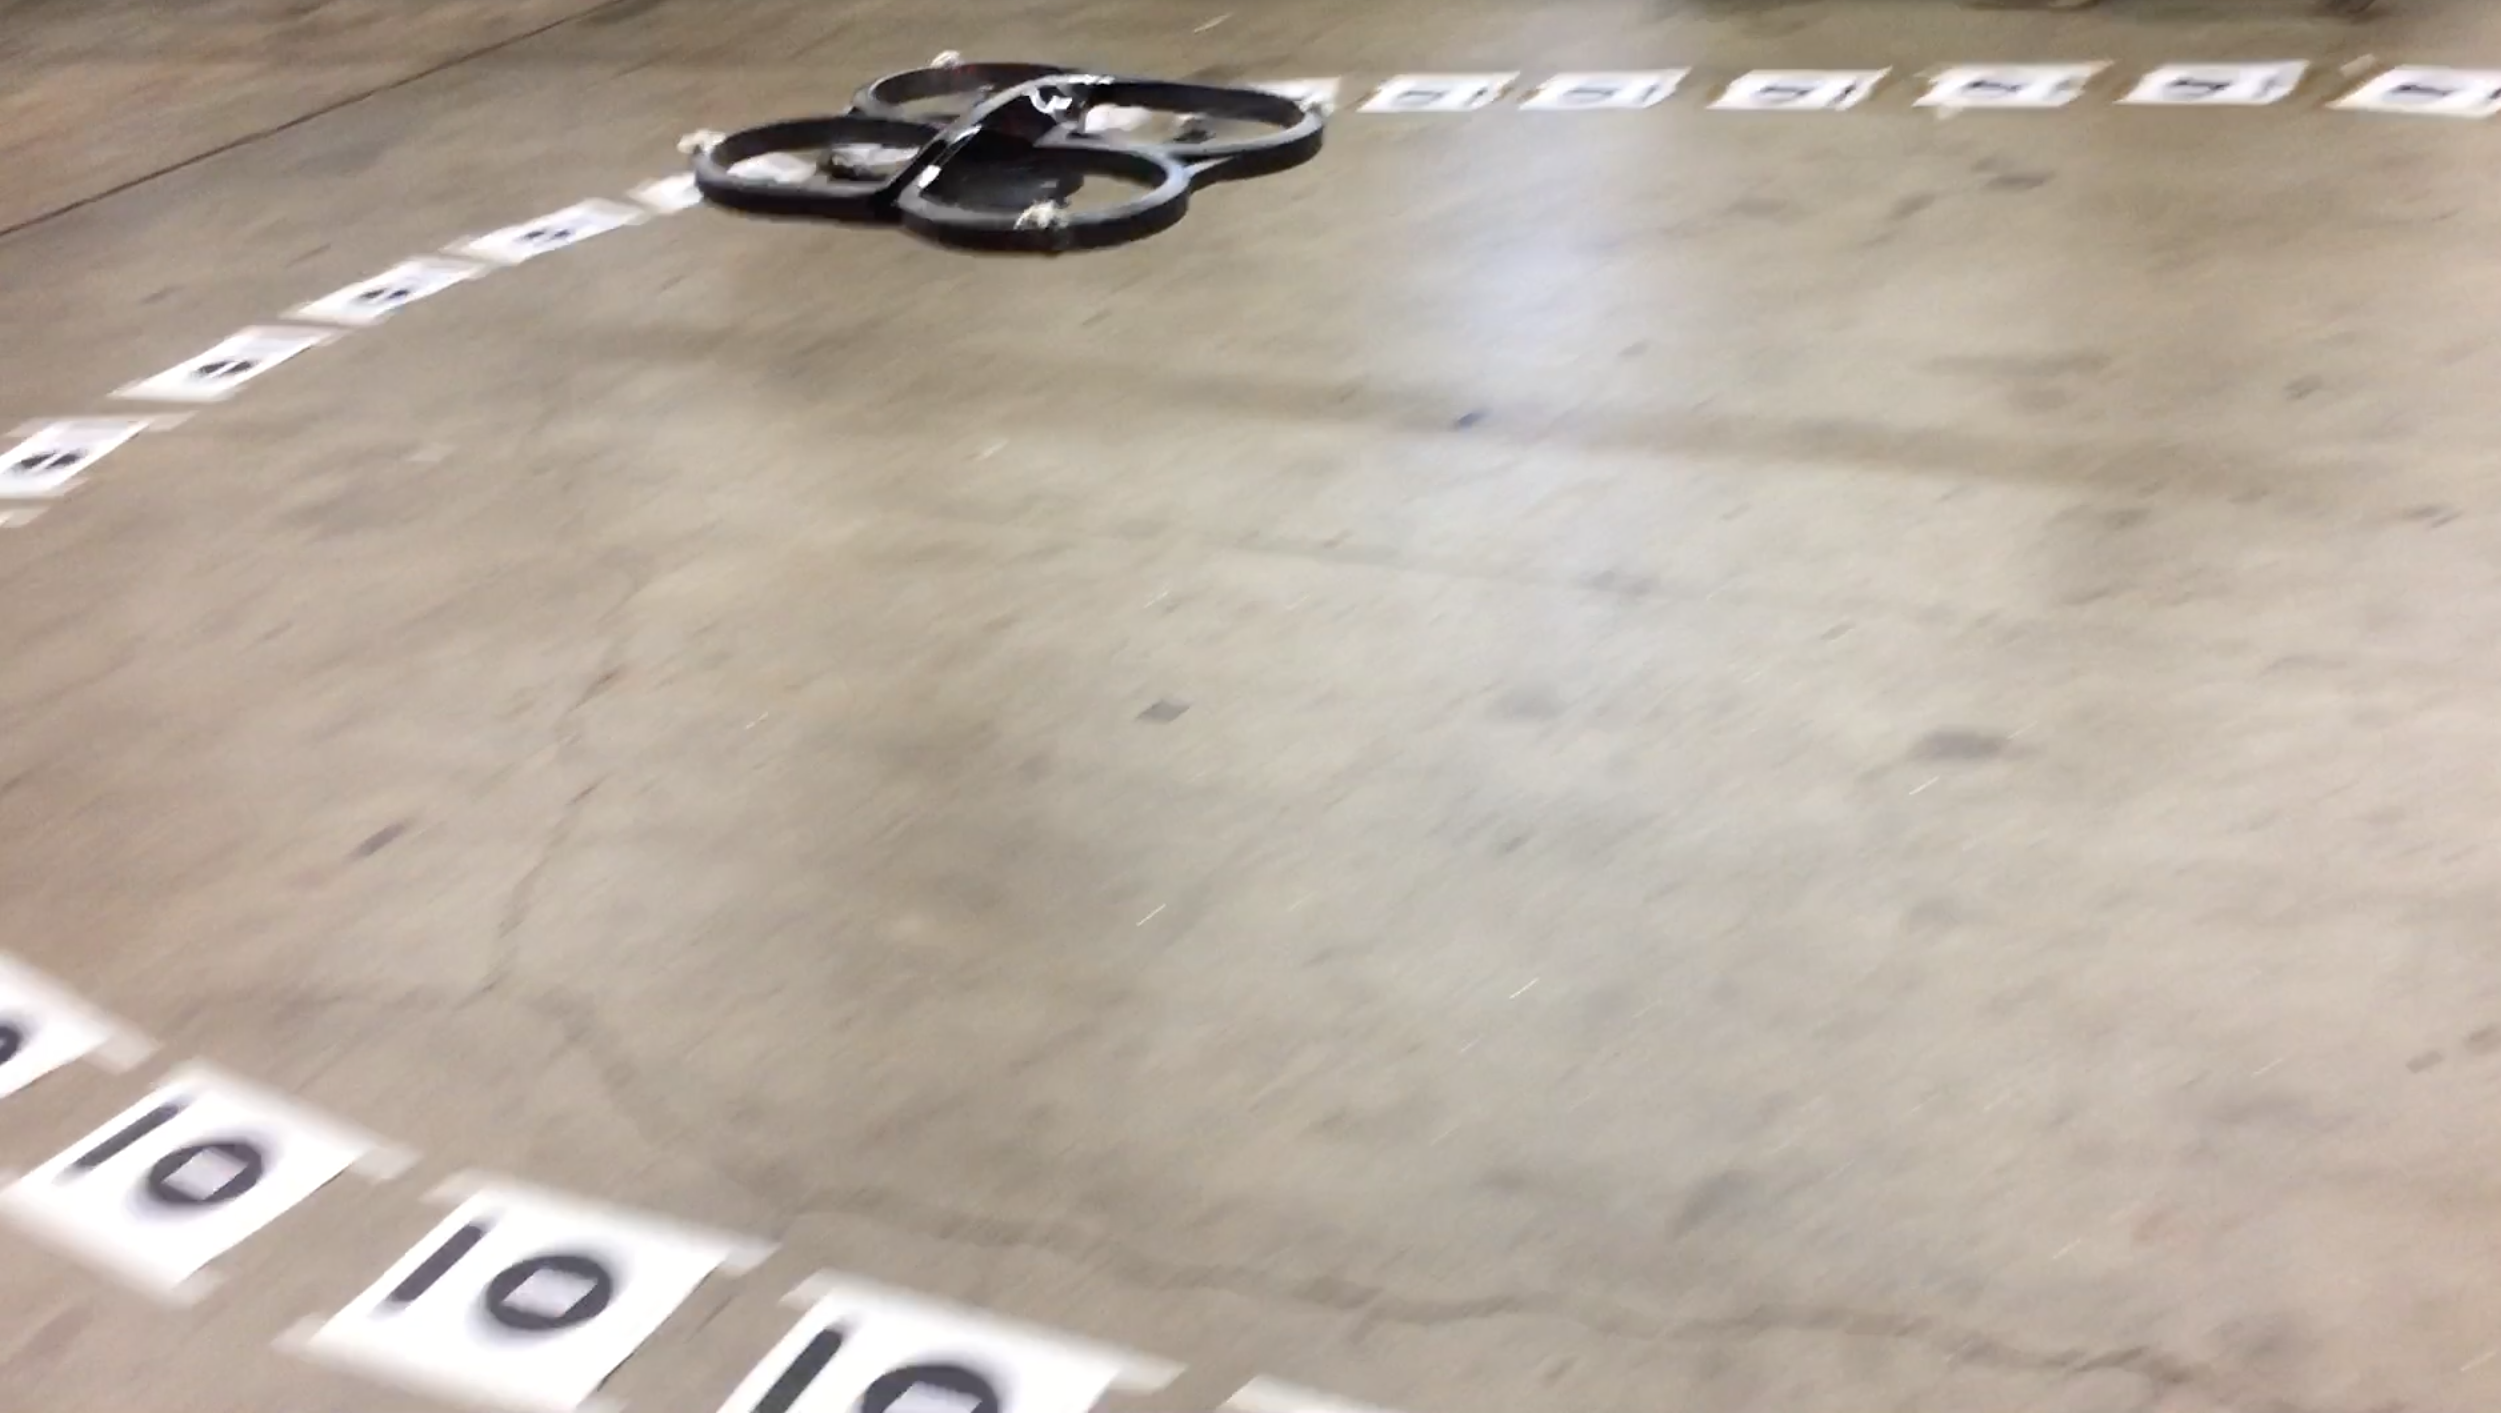
\includegraphics[width=\linewidth]{4c-backing-away.png}
                \caption{Drone is now backing away from the roundel}
        \end{subfigure}
        \caption{Screenshots from a video}\label{fig:4c-video}
\end{figure}
\twocolumn